\documentclass[a4paper,10pt]{report}

\usepackage{url}
\usepackage{graphics}
\usepackage{verbatim}
\usepackage{amsthm}

% Title Page
\title{Newick Utilities Tutorial}
\author{Thomas Junier}


\newcommand{\nutils}{Newick Utilities}
\newcommand{\unix}{\textsc{Unix}}
\newcommand{\ascii}{\textsc{ASCII}}
\newcommand{\svg}{\textsc{SVG}}
\newcommand{\stdin}{standard input}
\newcommand{\nw}{Newick}
\newcommand{\css}{\textsc{CSS}}

% names of programs
\newcommand{\display}{\texttt{nw\_display}}
\newcommand{\reroot}{\texttt{nw\_reroot}}
\newcommand{\topology}{\texttt{nw\_topology}}
\newcommand{\labels}{\texttt{nw\_labels}}

\newtheorem{prop}{Proposition}
\newtheorem{lemma}{Lemma}
\theoremstyle{definition}
\newtheorem{dfn}{Definition}

\begin{document}
\maketitle
\tableofcontents

\chapter{Introduction}

The \nutils{} are a set of \unix{} shell programs for working with Newick-formatted phylogenetic trees. Their main features are:
\begin{itemize}
 \item they require no user interaction.\footnote{Why this is a good thing is not the focus of this document: I shall assume that if you are reading this, you already know when a command-line interface is better than an interactive interface.}
 \item they can work on any number of trees at a time\footnote{Strictly speaking, a few applications are limited to one input tree because working on more than one is not practical}
 \item they perform reasonably well with large trees
 \item they are implemented as filters
\end{itemize}
They are not tools for \emph{making} phylogenies. Rather, they are for working with existing ones, by which I mean manipulating the tree or extracting information from it: rerooting, simplifying, extracting subtrees, printing branch lengths and distances, etc - a glance at the table of contents of this document should give you an idea.

Each of the programs performs one task (with some variants). For example, here is how you would reroot a series of phylograms contained in file \texttt{mytrees.nw} using node \texttt{Dmelano} as outgroup:

\begin{verbatim}
$ nw_reroot mytrees.nw Dmelano
\end{verbatim} 
Now, you might want to make cladograms from the rerooted trees. Program \topology{} does the job, and since the utilities are filters, you can do it in a single command:
\begin{verbatim}
$ nw_reroot mytrees.nw Dmelano | nw_topology -
\end{verbatim}
As you can see, it is straightforward to pipe \nutils{} together, and of course they can be mixed freely with any other shell tool (see e.g. \ref{sct_counting_leaves}).

This document is organized as follows: chapter \ref{chap_general} discusses common features of the \nutils, chapter \ref{chap_simple} shows examples of simple tasks, and chapter \ref{chap_adv} has examples of more advanced tasks. 

\chapter{General Remarks}
\label{chap_general}

The following applies to all programs in the \nutils{} package.

\section{Help}
\label{sect_help}

All programs print a help message if passed option \texttt{-h}:

\begin{samepage}
\begin{verbatim}
$ nw_indent -h
Indents the Newick, making structure more clear.

Synopsis
--------

nw_indent [-cht:] <newick trees filename|->

Input
-----

Argument is the name of a file that contains Newick trees, or '-' (in
which case trees are read from standard input).

Output
------

By default, prints the input tree, with each parenthesis and each leaf on a
line of its own, and indented a multiple of '  ' (two spaces) to reflect
structure. The default output is valid Newick.
[...]
\end{verbatim}
\end{samepage}
The help page describes the program's purpose, its input and output, and its options, in a format reminiscent of \unix{} manpages. It also shows a few examples. All examples can be tried out using files in the \texttt{data} directory.

\section{Input}
\label{sect_input}

Since the \nutils{} are for working with trees, it should not be a surprise that all programs take Newick as input. The Newick format is a file format for (phylogenetic) trees. It is one of the most widely used and uderstood formats.
A complete description can be found at \url{http://evolution.genetics.washington.edu/phylip/newicktree.html}.

The input tree(s) are always the first argument to the program (after any options). They may either be stored in a file, or piped on \stdin{}. In the latter case, the filename is replaced by a '\texttt{-}' (dash):

\begin{samepage}
\begin{verbatim}
$ nw_display mytrees.nw
\end{verbatim}
is the same as
\begin{verbatim}
$ cat mytrees.nw | nw_display -
\end{verbatim}
\end{samepage}
Of course the second form is only really useful when chaining several programs into pipelines.

\subsection{Multiple Trees in Input}

Most programs can work on any number of trees. That is, in the example above the file \texttt{mytrees.nw} may contain one or more trees, preferably one tree per line\footnote{It may also work if the trees are formatted differently, but the programs were only tested on input files with one tree per line.}. The task will be performed on each tree in the input. So if you need to reroot 1,000 trees on the same outgroup, you can do it all in a single step (see \ref{sct_reroot}).

\section{Output}
\label{sect_output}

The \nutils{} either modify trees and print the result, or print information about the trees. In the first case, the output is also Newick.

\chapter{Simple Tasks}
\label{chap_simple}

\section{Displaying Trees}
\label{sct_display}

Perhaps the simplest and most common operation on a \nw{} tree is just to look at it. The \nw{} format is not very easy to understand for us humans, so we have to produce a graphical representation from it. This is the purpose of the \display{} program. 

\subsection{As Text}
\label{sct_display_text}

At the simplest, \display{} just outputs a text graph:

\verbatiminput{dspl1_txt.cmd}
\verbatiminput{dspl1_txt.out}

That's pretty low-tech compared to interactive, colorful graphical displays, but if you use the shell a lot (like I do), you may find it useful.

You can use option \texttt{-w} (``width'') to set the number of columns available for display:

\verbatiminput{dspl2_txt.cmd}
\verbatiminput{dspl2_txt.out}

\subsection{As \svg}
\label{sct_display_svg}

First, a disclaimer: there are dozens of tools for viewing trees out there, and I'm not interested in competing with them. The reason why I added \svg{} capabilities were:
\begin{itemize}
 \item I wanted to be able to produce reasonable graphics even if no other tool was available
 \item I wanted to be sure that large trees could be rendered\footnote{I have had serious problems visualising trees of more than 1,000 leaves using some popular software I will not name here - either it was painfully slow, or it simply crashed} 
\end{itemize}

\noindent{}To produce \svg, pass option \texttt{-s}:
\begin{verbatim}
$ nw_display -s catarrhini > catarrhini.svg
\end{verbatim}

Now you can visualize the result using any \svg-enabled tool (all good Web browsers can do it), or convert it to another format with, say \texttt{rsvg} or Inkscape. The following image was produced like this:

\begin{verbatim}
$ inkscape -f catarrhini.svg -A catarrhini.pdf
\end{verbatim}

\begin{center}
 \includegraphics{dspl_svg1_svg.pdf}
\end{center}

There are many options for \svg{} graphs.First, you can make radial trees, using option \texttt{-r} (from now on I will skip the redirection into an \svg{} file):

\verbatiminput{dspl_sr_w450_catarrhini_svg.cmd}

You already know \texttt{-w}, except that for \svg{} the value is in pixels instead of columns. 

\begin{center}
\includegraphics{dspl_sr_w450_catarrhini_svg.pdf}
\end{center}

\subsubsection{Using \css}
\label{sct_display_svg_css}

You can modify node style using \css. This is done by specifying a \textit{\css{} map}, which is just a text file that says which style should be applied to which node. If file \texttt{css.map} contains the following
\begin{quote}
 \verbatiminput{css.map}
\end{quote} 
we can apply the style map to the tree above:

\verbatiminput{nw_display_sr_w450_ccssmap_catarrhini_svg.cmd}

\begin{center}
 \includegraphics{nw_display_sr_w450_ccssmap_catarrhini_svg.pdf}
\end{center}

The syntax of the \css{} map is as follows. Each line describes one style and the set of nodes to which it applies. The first line in \texttt{css.map} says that the style \texttt{stroke-width:2;stroke:blue} must be applied to the \texttt{CLADE} defined by \texttt{Homo} and \texttt{Pan}, which comprises \texttt{Homo}, \texttt{Pan}, and \texttt{Hominini}. The \texttt{CLADE} keyword can be abbreviated to \texttt{C}, as in the next two lines. The style of an inner clade overrides styles of an outer clade, \textit{e.g.}, although the \texttt{Homo} - \texttt{Pan} clade is nested inside the \texttt{Homo} - \texttt{Hylobates} clade, it has its own style (blue, wide lines) which overrides the containing clade's style (pinkish with normal width).

The \texttt{INDIV} keyword specifies that the style is to be applied to all nodes who match the labels on the line, but individually, that is, the program does not propagate the style to the whole clade defined by the labels. This is why only \texttt{Colobus} and \texttt{Cercopithecus} appear in green; with the \texttt{CLADE} keyword the whole \texttt{Macaca} - \texttt{Colobus} clade (that is, all Old-World monkeys) would be green. Note that \texttt{INDIV} overrides \texttt{CLADE}, which is why \texttt{Cercopithecus} is green even though it belongs to a red clade.

\section{Indenting}
\label{sct_indent}

\section{Rooting and Rerooting}
\label{sct_reroot}

Rooting transforms an unrooted tree into a rooted one, and rerooting changes a rooted tree's root. Some tree-building methods produce rooted trees (e.g., \textsc{UPGMA}), others produce unrooted ones (neighbor-joining, maximum-likelihood). 

The Newick format is implicitly rooted, in the sense that there is a 'top' node from which all other nodes descend. Some applications regard a tree with a trifuraction at the top node as unrooted. 

One way of (re)rooting a tree is to specify an \textit{outgroup}. In the simplest case, this is a single leaf. The root is then placed in such a way that one of its children is the outgroup, while the other child is the rest of the tree (sometimes known as the \textit{ingroup}). 

Consider the following primate tree, \texttt{simiiformes\_wrong}:

\includegraphics{reroot_1og_orig_svg.pdf}

\noindent{}It is wrong because \texttt{Cebus}, which is a New World monkey (capuchin), should be the sister group of all the rest (Old World monkeys and apes, technically Catarrhini), whereas it is shown as the sister group of the macaque-colobus family, Cercopithecidae. We can correct this by re-rooting the tree using \texttt{Cebus} as outgroup:
\verbatiminput{reroot_1og_corr_svg.cmd}
which produces:
\includegraphics{reroot_1og_corr_svg.pdf}

The outgroup does not need to be a single leaf. The following tree is wrong for the same reason as the one before, except that is has three New World monkey species instead of one, and they appear as a clade (Platyrrhini) in the wrong place:

\includegraphics{reroot_3og_orig_svg.pdf}

\noindent{}We can correct this by specifying the New World monkey clade as outgroup:

\verbatiminput{reroot_3og_result_svg.cmd}

\includegraphics{reroot_3og_result_svg.pdf}

\noindent{}Note that I did not include all three New World monkeys, only \texttt{Cebus} and \texttt{Allouatta}. This is because it is always possible to define a clade using only two leaves. The result would be the same if I had included all three, though. You can use inner labels too, if there are any:
\begin{verbatim}
$ nw_reroot simiiformes_wrong_3og Platyrrhini
\end{verbatim}
will reroot in the same way (not shown). Beware that inner labels are often used for support values (as in bootstrapping), which are generally not useful for defining clades.

\section{Extracting Labels}
\label{sct_labels}

To get a list of all labels in a tree, use \labels:

\verbatiminput{labels_xpl1_txt.cmd}
\verbatiminput{labels_xpl1_txt.out}

\noindent{}The labels are printed out in post-order. To get rid of internal labels, use \texttt{-I}:

\verbatiminput{labels_xpl2_txt.cmd}
\verbatiminput{labels_xpl2_txt.out}

\noindent{}Likewise, you can use \texttt{-L} to get rid of leaf labels (not shown). Finally, if you use \texttt{-t} the labels are printed on a single line, separated by tabs (for some reason the tabs show as spaces here, I think this is an effect of \LaTeX{}'s \verb+\verbatiminput{}+):

\verbatiminput{labels_xpl3_txt.cmd}
\verbatiminput{labels_xpl3_txt.out}

\subsection{Counting Leaves in a Tree}
\label{sct_counting_leaves}

A simple application of \labels{} is a leaf count:

\verbatiminput{labels_xpl4_txt.cmd}
\verbatiminput{labels_xpl4_txt.out}

\subsection{Extracting Subtrees}
\label{sct_subtrees}

You can extract subtrees (clades) as defined by labels (see \ref{sct_defining_clades}).

\chapter{More Elaborate Tasks}
\label{chap_adv}

\appendix

\chapter{Some Properties of Trees}
\label{sct_defining_clades}

\begin{figure}[t]
\centering
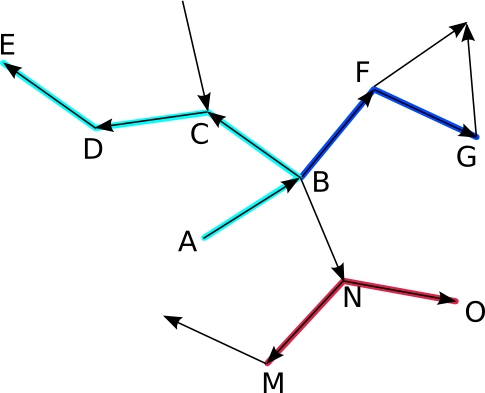
\includegraphics{oriented_graph.png}
 % oriented_graph.png: 485x393 pixel, 300dpi, 4.11x3.33 cm, bb=0 0 116 94
 \caption{An oriented graph (not a tree!), with edge orientation shown as arrows. Two paths are highlighted (cyan and blue). The cyan path starts at node A and ends at node E. Nodes B, C, D, and E are reachable from A. Node C is the direct successor of B in the cyan path; in the blue path the direct successor of B is F. The segment highlighted in red is \emph{not} a path.}
 \label{fig_oriented_graph}
\end{figure}



In the following, $T$ will be a rooted tree. We'll recall that a tree (rooted or not) is a connected, acyclic graph. By choosing one node to be the root (which we'll note $R$), and orienting all edges away from the root, we get an oriented graph. A \textit{path} along such a graph is a sequence of nodes such that there is an edge between two successive nodes, and that these nodes are ordered in the sequence as they are in the edge. The first node in the path is called the \textit{start} of the path, and the last node is its \textit{end}. We speak of a path \textit{from} the start \textit{to} the end, equivalently we say that the end is \textit{reachable} from the start. The nodes in a path are ordered: if $a$ and $b$ are in a path, then either $a$ is reachable from $b$, or $b$ is reachable from $a$, or $a = b$; furthermore if $a$ is reachable from $b$, then $b$ is \textit{not} reachable from $a$. If an edge connects $a$ to $b$, then $b$ is the \textit{direct successor} of $a$, and $a$ is the \textit{direct predecessor} of $b$
See figure {\ref{fig_oriented_graph}.

Although paths are not sets, we will (somewhat abusively, perhaps) use set notation with paths, unless there is a risk of confusion. Thus is $P$ is a path and $n$ is a node, then $n \in P$ means that $n$ is ``in'' $P$  or ``belongs to'' $P$ (strictly speaking, $n$ is reachable from the start of $P$, and the end of $P$ is reachable from $n$).

Now a few definitions - these are mostly renamings of graph-theoretical concepts, to make them more intuitive for phylogenetic trees. 

\begin{dfn}
\label{def_ancestor}
Let $a$ and $b$ be two different nodes of $T$. We say that $a$ is an \textit{ancestor} of $b$, or (equivalently) that $b$ is a \textit{descendant} of $a$, if and only if there is a path from $a$ to $b$. 
\end{dfn}

\begin{dfn}
\label{def_parent}
Let $P$ be a path in $T$, and $a, b$ two nodes in $P$ such that $b$ is the direct successor of $a$. We will call $a$ the \textit{parent} of $b$. We can say \textit{the} parent (rather than \textit{a} parent) of $b$ because i) $a$ lies on the path from $R$ to $b$ (which is unique), and ii) only one node on any path can be another node's direct predecessor. We also see that any node's parent is also its ancestor (which shouldn't be too surprising\ldots), since $b$ is reachable from $a$
\end{dfn}

\begin{dfn}
\label{def_child}
Let $P$ be a path in $T$, and $a, b$ two nodes in $P$ such that $b$ is the direct successor of $a$. We say that $b$ is a \textit{child} of $a$.
\end{dfn}

Note that a node has exactly one parent, except the root which has none. A node can have zero or more children, but we rarely ever encounter nodes with a single child. A node with no children is called a \textit{leaf}.

\begin{dfn}
\label{def_lineage}
A path that starts from the root we call a \emph{lineage}. By the definition of a rooted tree, there is always a lineage to $n$ for any node $n$, and this lineage is unique. So we can unambiguously talk of \textit{the} lineage of $n$ to mean the path from $R$ to $n$. We say that a set $L$ of nodes form a lineage if there exists $n \in L$ such that the path from $R$ to $n$ contains all and only elements of $L$.
\end{dfn}

\begin{figure}[b]
 \centering
 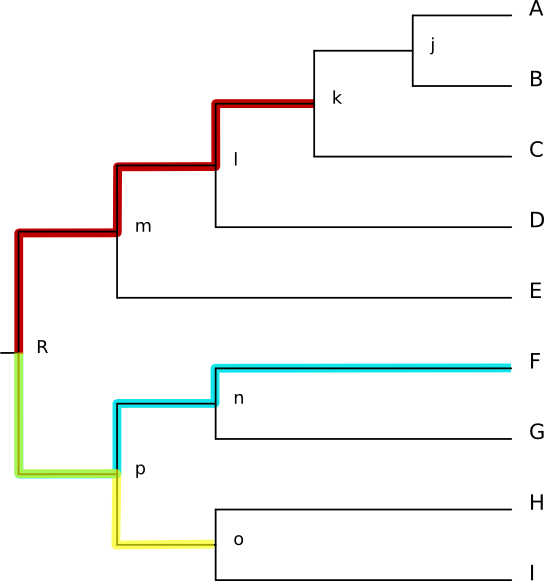
\includegraphics{prop_tree.png}
  \caption{A rooted tree}
 \label{fig_app_tree_prop}
\end{figure}

\begin{prop}
\label{prop_lineage_ancestors_equivalence}
Let $n$ be a node of $T$, and $L$ its lineage. Then all ancestors of $n$ belong to $L$, and all nodes of $L$, except $n$ itself, are ancestors of $n$.
\end{prop}

\begin{proof}

$\Rightarrow$ Let $a$ be an ancestor of $n$. By definition \ref{def_ancestor}, there is a path from $a$ to $n$. By tree properties, there is a path from $R$ to $a$. Hence $a$ belongs to the path from $R$ to $n$, which is the lineage of $n$.
\end{proof}

\noindent{}$\Leftarrow$ Let $l \neq n$ be a node in $L$. Since $L$ is the path from $R$ to $n$, $n$ is reachable from $a$, and hence $a$ is an ancestor of $n$ by definition \ref{def_ancestor}.

\begin{dfn}
If $L$ and $M$ are lineages of $T$, then the \textit{intersection}
of $L$ and $M$, noted $L \cap M$, is the set of nodes that belong to both $L$ and $M$.
\end{dfn} 

\begin{lemma}
\label{lem_ancestors_in_lineage}
Let $n$ be a node of $T$, $L$ its lineage, and $l$ a node of $L$. Then $l$'s ancestors also belong to $L$.
\end{lemma}
\begin{proof}
If $l = n$ then the ancestors of $l$ are those of $n$, which belong to $L$ by proposition \ref{prop_lineage_ancestors_equivalence}. If $l \neq n$ then let $a$ be an ancestor of $l$. By definition \ref{def_ancestor}, $l$ is reachable from $a$. By proposition \ref{prop_lineage_ancestors_equivalence}, $l$ is an ancestor of $n$ and again $n$ is reachable from $l$. Therefore, $n$ is reachable from $a$, so $a$ is an ancestor of $n$, and so belongs in $L$.
\end{proof}

\begin{lemma}
Let $L$ and $M$ be lineages of $T$, and $q \in L \cap M, q \neq R$. Then $q$'s parent also belongs to $M \cap L$.
\end{lemma}
\begin{proof}
Call $p$ the parent of $q$. $p$ is an ancestor of $q$, and since $q$ belongs to $L$ (by hypothesis), $p$ belongs to $L$ by lemma \ref{lem_ancestors_in_lineage}. By the same reasoning, $p$ belongs to $M$, therefore $p \in L \cap M$.

\end{proof}


\begin{prop}
\label{prop_lineage_intersection}
Let $L$ and $M$ be lineages of $T$. Then $L \cap M$ also forms a lineage.
\end{prop}
\begin{proof}
Let $N = L \cap M$. Because $N$ is a subset of a lineage (in fact it is a subset of at least two lineages, $L$ and $M$), its elements are ordered, so we can pick the last one and call it $n$. Now all other elements of $N$ are ancestors of $n$, so by lemma \ref{lem_ancestors_in_lineage} they belong in $L$ and in $M$. So far we have proven 
\end{proof}



\begin{prop}
In a rooted tree, you can always define a clade by specifying a single node: the clade consists of the specified node and all its descendants.
\end{prop}

\begin{prop}
In a rooted tree $T$ with unique labels and a node $n$ in $T$, it is always possible to choose two nodes $n_1$ and $n_2$ such that lca($n_1$,$n_2$) = $n$.
\end{prop}

\end{document}
